\documentclass[conference]{IEEEtran}
\IEEEoverridecommandlockouts
\usepackage{cite}
\usepackage{amsmath,amssymb,amsfonts}
\usepackage{graphicx}
\usepackage{booktabs}
\usepackage{multirow}
\usepackage{textcomp}
\usepackage{xcolor}
\usepackage{tikz}
\usetikzlibrary{arrows.meta,positioning,fit,backgrounds}
\usepackage{hyperref}

\begin{document}

\title{Attention Is All You Need}

\author{%
\IEEEauthorblockN{Ashish Vaswani\thanks{Equal contribution. Listing order is random.}\quad Noam Shazeer\footnotemark[1]\quad Niki Parmar\footnotemark[1]\quad Jakob Uszkoreit\footnotemark[1]}
\IEEEauthorblockA{\textit{Google Brain / Google Research} \\
\{avaswani, noam, nikip, usz\}@google.com}
\and
\IEEEauthorblockN{Llion Jones\footnotemark[1]\quad Aidan N. Gomez\footnotemark[1]\quad {\L}ukasz Kaiser\footnotemark[1]\quad Illia Polosukhin\footnotemark[1]}
\IEEEauthorblockA{\textit{Google Research / University of Toronto} \\
llion@google.com,\ aidan@cs.toronto.edu}
}

\maketitle

\begin{abstract}
The dominant sequence transduction models are based on complex recurrent or
convolutional neural networks that include an encoder and a decoder. The best
performing models also connect the encoder and decoder through an attention
mechanism. We propose a new simple network architecture, the Transformer, based
solely on attention mechanisms, dispensing with recurrence and convolutions
entirely. Experiments on two machine translation tasks show these models to be
superior in quality while being more parallelizable and requiring significantly
less time to train. Our model achieves 28.4 BLEU on the WMT 2014 English-to-German
translation task, improving over the existing best results, including ensembles,
by over 2 BLEU. On the WMT 2014 English-to-French translation task, our model
establishes a new single-model state-of-the-art BLEU score of 41.8 after training
for 3.5 days on eight GPUs, a small fraction of the training costs of the best
models from the literature.
\end{abstract}

\begin{IEEEkeywords}
attention, self-attention, sequence transduction, neural machine translation, Transformer
\end{IEEEkeywords}

\section{Introduction}
Recurrent neural networks, long short-term memory~\cite{hochreiter1997} and gated
recurrent~\cite{cho2014} neural networks in particular, have been firmly
established as state-of-the-art approaches in sequence modeling and transduction
problems such as language modeling and machine translation. Recurrent models
typically factor computation along the symbol positions of the input and output
sequences. Aligning the positions to steps in computation time, they generate a
sequence of hidden states $h_t$, as a function of the previous hidden state
$h_{t-1}$ and the input for position $t$. This inherently sequential nature
precludes parallelization within training examples, which becomes critical at
longer sequence lengths, as memory constraints limit batching across examples.

Attention mechanisms have become an integral part of compelling sequence modeling
and transduction models, allowing modeling of dependencies without regard to
their distance in the input or output sequences~\cite{bahdanau2015}. In this work
we propose the Transformer, a model architecture eschewing recurrence and instead
relying entirely on an attention mechanism to draw global dependencies between
input and output. The Transformer allows for significantly more parallelization
and can reach a new state of the art in translation quality after being trained
for as little as twelve hours on eight P100 GPUs.

\section{Background}
The goal of reducing sequential computation also forms the foundation of the
Extended Neural GPU, ByteNet~\cite{kalchbrenner2016} and
ConvS2S~\cite{gehring2017}, all of which use convolutional neural networks as a
basic building block. In these models the number of operations required to relate
signals from two arbitrary input or output positions grows in the distance
between positions, linearly for ConvS2S and logarithmically for ByteNet. In the
Transformer this is reduced to a constant number of operations, albeit at the cost
of reduced effective resolution due to averaging attention-weighted positions, an
effect we counteract with multi-head attention.

Self-attention, sometimes called intra-attention, is an attention mechanism
relating different positions of a single sequence in order to compute a
representation of the sequence. Self-attention has been used successfully in a
variety of tasks including reading comprehension, abstractive summarization, and
learning task-independent sentence representations~\cite{cheng2016,lin2017}. To
the best of our knowledge, however, the Transformer is the first transduction
model relying entirely on self-attention to compute representations of its input
and output without using sequence-aligned RNNs or convolution.

\section{Model Architecture}
Most competitive neural sequence transduction models have an encoder-decoder
structure~\cite{sutskever2014}. Here, the encoder maps an input sequence of symbol
representations $(x_1, \dots, x_n)$ to a sequence of continuous representations
$\mathbf{z} = (z_1, \dots, z_n)$. Given $\mathbf{z}$, the decoder then generates
an output sequence $(y_1, \dots, y_m)$ of symbols one element at a time. At each
step the model is auto-regressive, consuming the previously generated symbols as
additional input when generating the next.

The Transformer follows this overall architecture using stacked self-attention
and point-wise, fully connected layers for both the encoder and decoder, shown in
the two halves of Fig.~\ref{fig:arch}.

\begin{figure}[t]
\centering
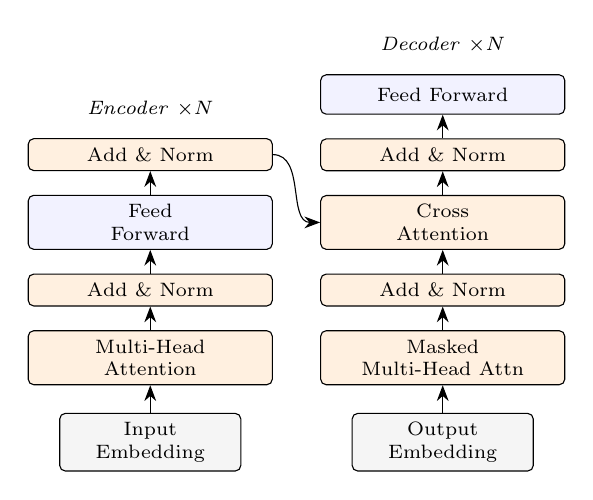
\begin{tikzpicture}[
  font=\scriptsize,
  box/.style={draw, rounded corners=2pt, minimum width=3.1cm, minimum height=0.5cm, align=center, fill=blue!5},
  addn/.style={draw, rounded corners=2pt, minimum width=3.1cm, minimum height=0.4cm, align=center, fill=orange!12},
  emb/.style={draw, rounded corners=2pt, minimum width=2.3cm, minimum height=0.45cm, align=center, fill=gray!8},
  >={Stealth[length=2mm]}
]
% Encoder stack
\node[emb] (ei) {Input\\Embedding};
\node[addn, above=0.35cm of ei] (ea1) {Multi-Head\\Attention};
\node[addn, above=0.3cm of ea1] (ea2) {Add \& Norm};
\node[box, above=0.3cm of ea2] (ef) {Feed\\Forward};
\node[addn, above=0.3cm of ef] (ea3) {Add \& Norm};
\draw[->] (ei) -- (ea1);
\draw[->] (ea1) -- (ea2);
\draw[->] (ea2) -- (ef);
\draw[->] (ef) -- (ea3);
\node[above=0.15cm of ea3] {\textit{Encoder} $\times N$};

% Decoder stack
\node[emb, right=1.4cm of ei] (di) {Output\\Embedding};
\node[addn, above=0.35cm of di] (da1) {Masked\\Multi-Head Attn};
\node[addn, above=0.3cm of da1] (da2) {Add \& Norm};
\node[addn, above=0.3cm of da2] (dx) {Cross\\Attention};
\node[addn, above=0.3cm of dx] (da3) {Add \& Norm};
\node[box, above=0.3cm of da3] (df) {Feed Forward};
\draw[->] (di) -- (da1);
\draw[->] (da1) -- (da2);
\draw[->] (da2) -- (dx);
\draw[->] (dx) -- (da3);
\draw[->] (da3) -- (df);
\draw[->] (ea3.east) to[out=0,in=180] (dx.west);
\node[above=0.15cm of df] {\textit{Decoder} $\times N$};
\end{tikzpicture}
\caption{The Transformer follows an encoder-decoder structure built from stacked
self-attention and point-wise feed-forward layers. The decoder additionally
attends over the encoder output (cross attention).}
\label{fig:arch}
\end{figure}

\subsection{Encoder and Decoder Stacks}
\textbf{Encoder.} The encoder is composed of a stack of $N = 6$ identical layers.
Each layer has two sub-layers. The first is a multi-head self-attention mechanism,
and the second is a simple, position-wise fully connected feed-forward network. We
employ a residual connection around each of the two sub-layers, followed by layer
normalization~\cite{ba2016}. That is, the output of each sub-layer is
$\mathrm{LayerNorm}(x + \mathrm{Sublayer}(x))$. All sub-layers, as well as the
embedding layers, produce outputs of dimension $d_{\text{model}} = 512$.

\textbf{Decoder.} The decoder is also composed of a stack of $N = 6$ identical
layers. In addition to the two sub-layers in each encoder layer, the decoder
inserts a third sub-layer, which performs multi-head attention over the output of
the encoder stack. We also modify the self-attention sub-layer in the decoder
stack to prevent positions from attending to subsequent positions. This masking,
combined with the fact that the output embeddings are offset by one position,
ensures that the predictions for position $i$ can depend only on the known outputs
at positions less than $i$.

\subsection{Attention}
An attention function can be described as mapping a query and a set of key-value
pairs to an output, where the query, keys, values, and output are all vectors. The
output is computed as a weighted sum of the values, where the weight assigned to
each value is computed by a compatibility function of the query with the
corresponding key.

\textbf{Scaled Dot-Product Attention.} We compute the dot products of the query
with all keys, divide each by $\sqrt{d_k}$, and apply a softmax function to obtain
the weights on the values. In practice, we compute the attention function on a set
of queries simultaneously, packed together into a matrix $Q$. The keys and values
are also packed together into matrices $K$ and $V$:
\begin{equation}
\mathrm{Attention}(Q, K, V) = \mathrm{softmax}\!\left(\frac{QK^{\top}}{\sqrt{d_k}}\right)V.
\label{eq:sdpa}
\end{equation}
While for small values of $d_k$ additive and dot-product attention perform
similarly, dot-product attention is much faster and more space-efficient in
practice. We suspect that for large values of $d_k$ the dot products grow large in
magnitude, pushing the softmax function into regions where it has extremely small
gradients. To counteract this effect, we scale the dot products by
$\frac{1}{\sqrt{d_k}}$.

\textbf{Multi-Head Attention.} Instead of performing a single attention function
with $d_{\text{model}}$-dimensional keys, values, and queries, we found it
beneficial to linearly project the queries, keys, and values $h$ times with
different, learned linear projections. On each of these projected versions we then
perform the attention function in parallel and concatenate the results:
\begin{equation}
\mathrm{MultiHead}(Q, K, V) = \mathrm{Concat}(\mathrm{head}_1, \dots, \mathrm{head}_h)W^{O},
\label{eq:mha}
\end{equation}
\begin{equation}
\text{where } \mathrm{head}_i = \mathrm{Attention}(QW_i^{Q}, KW_i^{K}, VW_i^{V}).
\end{equation}
In this work we employ $h = 8$ parallel attention heads. For each we use
$d_k = d_v = d_{\text{model}}/h = 64$. Due to the reduced dimension of each head,
the total computational cost is similar to that of single-head attention with full
dimensionality.

\subsection{Position-wise Feed-Forward Networks}
In addition to attention sub-layers, each layer contains a fully connected
feed-forward network, applied to each position separately and identically. This
consists of two linear transformations with a ReLU activation in between:
\begin{equation}
\mathrm{FFN}(x) = \max(0, xW_1 + b_1)W_2 + b_2.
\label{eq:ffn}
\end{equation}
The dimensionality of input and output is $d_{\text{model}} = 512$, and the inner
layer has dimensionality $d_{ff} = 2048$.

\subsection{Positional Encoding}
Since our model contains no recurrence and no convolution, in order for the model
to make use of the order of the sequence we inject information about the relative
or absolute position of the tokens. We add positional encodings to the input
embeddings, using sine and cosine functions of different frequencies:
\begin{align}
PE_{(pos, 2i)}   &= \sin\!\left(pos / 10000^{2i/d_{\text{model}}}\right),\\
PE_{(pos, 2i+1)} &= \cos\!\left(pos / 10000^{2i/d_{\text{model}}}\right),
\end{align}
where $pos$ is the position and $i$ is the dimension.

\section{Why Self-Attention}
In this section we compare various aspects of self-attention layers to the
recurrent and convolutional layers commonly used for mapping one variable-length
sequence of symbol representations to another. Motivating our use of
self-attention we consider three desiderata: the total computational complexity
per layer; the amount of computation that can be parallelized, as measured by the
minimum number of sequential operations required; and the path length between
long-range dependencies in the network. Table~\ref{tab:complexity} summarizes
these for the different layer types.

\begin{table*}[t]
\centering
\caption{Maximum path lengths, per-layer complexity, and minimum number of
sequential operations for different layer types. $n$ is the sequence length, $d$
the representation dimension, $k$ the kernel size, and $r$ the neighborhood size
in restricted self-attention.}
\label{tab:complexity}
\begin{tabular}{@{}lccc@{}}
\toprule
Layer Type & Complexity per Layer & Sequential Operations & Maximum Path Length \\
\midrule
Self-Attention             & $O(n^2 \cdot d)$        & $O(1)$ & $O(1)$ \\
Recurrent                  & $O(n \cdot d^2)$        & $O(n)$ & $O(n)$ \\
Convolutional              & $O(k \cdot n \cdot d^2)$ & $O(1)$ & $O(\log_k n)$ \\
Self-Attention (restricted) & $O(r \cdot n \cdot d)$  & $O(1)$ & $O(n/r)$ \\
\bottomrule
\end{tabular}
\end{table*}

\section{Training}
We trained on the standard WMT 2014 English-German dataset consisting of about 4.5
million sentence pairs, and the significantly larger WMT 2014 English-French
dataset consisting of 36M sentences. We trained our models on one machine with
eight NVIDIA P100 GPUs. For our base models, each training step took about 0.4
seconds, and we trained for a total of 100{,}000 steps or 12 hours. We used the
Adam optimizer~\cite{kingma2015} with $\beta_1 = 0.9$, $\beta_2 = 0.98$, and
$\epsilon = 10^{-9}$, and varied the learning rate over training according to a
warmup schedule. We applied residual dropout and label smoothing of
$\epsilon_{ls} = 0.1$ for regularization.

\section{Results}
\subsection{Machine Translation}
On the WMT 2014 English-to-German translation task, the big Transformer model
outperforms the best previously reported models, including ensembles, by more than
2.0 BLEU, establishing a new state-of-the-art BLEU score of 28.4. On the WMT 2014
English-to-French task, our big model achieves a BLEU score of 41.8, outperforming
all previously published single models at less than a quarter of the training cost
of the previous state-of-the-art model. Table~\ref{tab:bleu} summarizes our
results and compares translation quality and training costs to other model
architectures.

\begin{table*}[t]
\centering
\caption{The Transformer achieves better BLEU scores than previous
state-of-the-art models on the English-to-German and English-to-French
newstest2014 tests at a fraction of the training cost.}
\label{tab:bleu}
\begin{tabular}{@{}lccc@{}}
\toprule
 & \multicolumn{2}{c}{BLEU} & Training Cost (FLOPs) \\
\cmidrule(lr){2-3}
Model & EN-DE & EN-FR & \\
\midrule
ByteNet                 & 23.75 & --    & --                  \\
GNMT + RL               & 24.6  & 39.92 & $1.4 \times 10^{20}$ \\
ConvS2S                 & 25.16 & 40.46 & $1.5 \times 10^{20}$ \\
GNMT + RL Ensemble      & 26.30 & 41.16 & $1.8 \times 10^{21}$ \\
ConvS2S Ensemble        & 26.36 & 41.29 & $1.2 \times 10^{21}$ \\
\midrule
Transformer (base)      & 27.3  & 38.1  & $3.3 \times 10^{18}$ \\
\textbf{Transformer (big)} & \textbf{28.4} & \textbf{41.8} & $2.3 \times 10^{19}$ \\
\bottomrule
\end{tabular}
\end{table*}

\subsection{Model Variations}
To evaluate the importance of different components of the Transformer, we varied
our base model in different ways, measuring the change in performance on
English-to-German translation. Table~\ref{tab:variations} presents these results.
In rows (A) we vary the number of attention heads and the attention key and value
dimensions, keeping the amount of computation constant. Single-head attention is
0.9 BLEU worse than the best setting, but quality also drops off with too many
heads.

\begin{table}[t]
\centering
\caption{Variations on the Transformer architecture. Unlisted values are identical
to those of the base model. All metrics are on the English-to-German development
set, newstest2013.}
\label{tab:variations}
\begin{tabular}{@{}clcccc@{}}
\toprule
 & & $h$ & $d_k$ & $d_v$ & BLEU \\
\midrule
base & & 8  & 64 & 64 & 25.8 \\
\midrule
\multirow{2}{*}{(A)} & & 1  & 512 & 512 & 24.9 \\
                     & & 16 & 32  & 32  & 25.8 \\
\midrule
(B) & fewer $d_k$        & 8 & 16 & 16 & 25.1 \\
(C) & bigger model       & 8 & 64 & 64 & 26.2 \\
(D) & dropout $0.0$      & 8 & 64 & 64 & 24.6 \\
\bottomrule
\end{tabular}
\end{table}

\section{Conclusion}
In this work we presented the Transformer, the first sequence transduction model
based entirely on attention, replacing the recurrent layers most commonly used in
encoder-decoder architectures with multi-head self-attention. For translation
tasks, the Transformer can be trained significantly faster than architectures
based on recurrent or convolutional layers. On both WMT 2014 English-to-German and
English-to-French translation tasks we achieve a new state of the art. We are
excited about the future of attention-based models and plan to apply them to other
tasks and to input and output modalities other than text.

\bibliographystyle{IEEEtran}
\bibliography{refs}

\end{document}
